\documentclass[11pt]{beamer}
\usepackage[utf8]{inputenc}
\usepackage[croatian]{babel}
\usepackage{amsmath}
\usepackage{amsfonts}
\usepackage{amssymb}
\usepackage{graphicx}
\usetheme{CambridgeUS}
\begin{document}
  \author{Lovre Mrčela}
  \title[Harmonijska analiza glazbe]{Harmonijska analiza glazbe\\korištenjem valićne transformacije}
  \institute[FER]{Sveučilište u Zagrebu\\Fakultet elektrotehnike i računarstva}
  \date{17. siječnja 2017.}
  \setbeamercovered{transparent}
  \setbeamertemplate{navigation symbols}{}
  \frame[plain]{\maketitle}
  
  \AtBeginSection[]
  {
    \begin{frame}
      \frametitle{Sadržaj}
      \tableofcontents[currentsection]
    \end{frame}
  }

  \section{Uvod}
  
  \subsection{Glazbeni pojmovi}
  \begin{frame}
    \frametitle{Glazbeni ton}
    Svojstva tona:
    \begin{itemize}
      \item visina
      \item trajanje
      \item glasnoća
      \item boja
    \end{itemize}
    \vspace{10pt}
    U užem smislu: ton = visina tona.
  \end{frame}

  \begin{frame}
    \frametitle{Sadržaj glazbe}
    \begin{description}
      \item[Homofona glazba] melodija + pratnja
      \item[Polifona glazba] više samostalnih melodija
    \end{description}
  \end{frame}

  \begin{frame}
    \frametitle{Analiza glazbenog sadržaja}
    Vrste analize:
    \begin{itemize}
      \item \alt<1>{melodijska}{\textbf{melodijska}}
      \item \alt<1>{harmonijska}{\textbf{harmonijska}}
      \item polifonijska
      \pause
    \end{itemize}
  \end{frame}

  \begin{frame}
    \frametitle{Nazivi tonova}
    Slova abecede: $a, h, c, d, e, f, g$.\\
    \vspace{10pt}
    Povišen ton za pola: $\sharp$, snižen ton za pola: $\flat$.\\
    \vspace{10pt}
    Raspon od 8 tonova -- oktava.    
  \end{frame}

  \begin{frame}
    \frametitle{Akord i tonalitet}
    \begin{description}
      \item[akord] istovremeno zvučanje barem 3 tona različitih visina
      \item[tonalitet] skup tonova od kojih se sastoji melodija
    \end{description}
  
    Temeljni ton.\\
    \vspace{10pt}
    Vrsta: dur, mol.
  \end{frame}

  \subsection{Cilj}
  \begin{frame}
    \frametitle{Cilj}
    Računalna obrada glazbenog isječka u svrhu dobivanja korisne informacije:
    \begin{itemize}
      \item tonalitet
      \item akord
      \item melodija
    \end{itemize}
  \end{frame}

  \begin{frame}
    \frametitle{Uloga valićne transformacije}
    Format snimljene glazbe na računalu: 1D-signal zvučnog vala.\\
    \vspace{10pt}
    Ljudska percepcija glazbe: tonovi različitih visina (i boja) u vremenu.\\
    \vspace{10pt}
    Zaključak: potrebna je bolja reprezentacija snimljene glazbe kako bi se mogla otkriti neka informacija.
  \end{frame}

  \section{Valićna analiza}
  \begin{frame}
    \frametitle{Oblik korištenog valića}
    `Bump' valić iz \textsc{Matlab}-ovog \textit{wavelet} paketa:
    $$ \Psi\left( a \omega \right) = \exp\left( 1 - \frac{1}{1 - \frac{\left(a \omega - \mu \right)^2}{\sigma^2}} \right)_{\left[ \frac{\mu - \sigma}{a}, \frac{\mu + \sigma}{a} \right]} $$
    
    Raspon skala: prilagođen frekvencijama standardnih tonova.\\
    \vspace{10pt}
    Računanje postupkom u frekvencijskoj domeni.
  \end{frame}

  \section{Problemi u rekonstrukciji odsviranih tonova}
  \begin{frame}
    \frametitle{Problemi u rekonstrukciji odsviranih tonova}
    Jedan ton $\ne$ jedna frekvencija.\\
    \vspace{10pt}
    Problemi s očitavanjem odsviranih tonova:
    \begin{itemize}
      \item \textit{alikvoti} -- razmazivanje u frekvencijama
      \item ADSR ovojnica -- razmazivanje u vremenu
    \end{itemize}
  \end{frame}
  
  \subsection{\protect\textit{Alikvoti}}
  \begin{frame}
    \frametitle{\textit{Alikvoti}}
    Posljedica rezoniranja dijelova instrumenta.\\
    \vspace{10pt}
    Frekvencija $n$-tog alikvota: $f_n = n \cdot f_0$.\\
    \vspace{10pt}
    Dodatan problem: neke frekvencije nisu točno pogođene korištenom skalom.
  \end{frame}
  \begin{frame}
    \frametitle{\textit{Alikvoti}}
    \begin{figure}
      \centering
      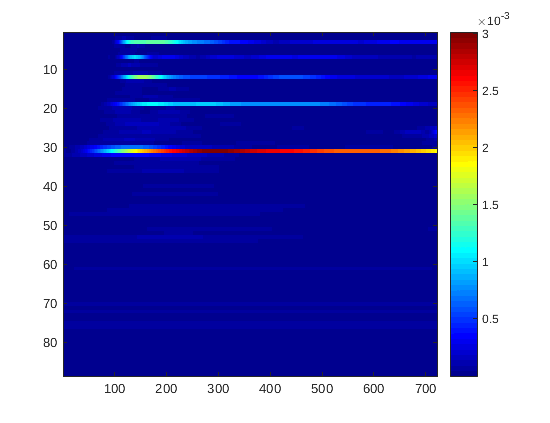
\includegraphics[height=0.9\textheight]{alikvoti.png}
    \end{figure}
  \end{frame}
    
  \begin{frame}
    \frametitle{\textit{Alikvoti}}
    Uklanjanje nije potrebno -- robusnost algoritma:
    \begin{itemize}
      \item ekstrakcija tonaliteta i akorda: većina \textit{alikvotnih} frekvencija ne smeta,
      \item ekstrakcija melodije: najniža frekvencija je temeljna.
    \end{itemize}
  \end{frame}
  
  \subsection{ADSR ovojnica}
  \begin{frame}
    \frametitle{ADSR ovojnica}
    Attack-Decay-Sustain-Release: opisuje oblik amplitude odsviranog tona.\\
    \vspace{10pt}
    \begin{figure}
      \centering
      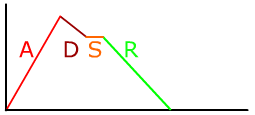
\includegraphics[height=0.4\textheight]{Adsr3.png}
    \end{figure}
  \end{frame}
  
  \begin{frame}
    \frametitle{ADSR ovojnica}
    Problem: određivanje koji tonovi zvuče istovremeno.
    \begin{figure}
      \centering
      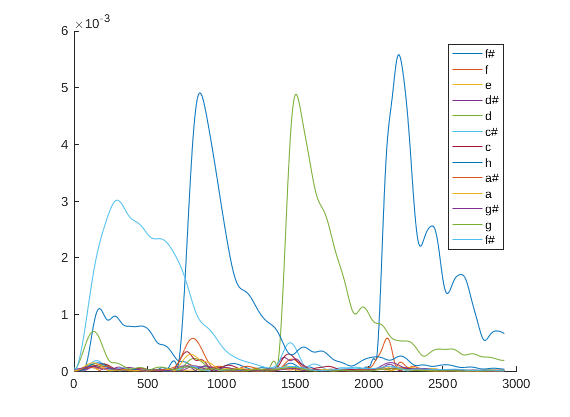
\includegraphics[height=0.8\textheight]{adsr_anomalija.png}
    \end{figure}
  \end{frame}
  
  \begin{frame}
    \frametitle{ADSR ovojnica}
    Zgodno rješenje: derivacija.
    \begin{figure}
      \centering
      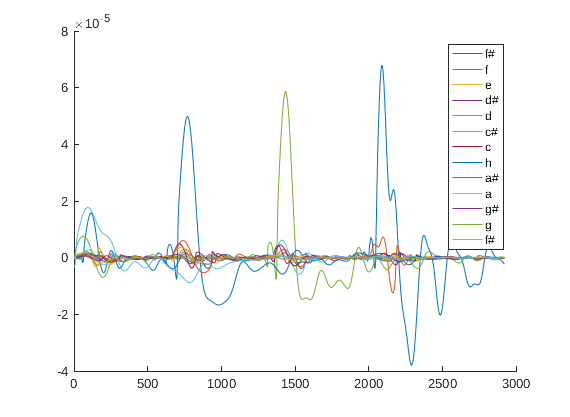
\includegraphics[height=0.8\textheight]{adsr_der.png}
    \end{figure}
  \end{frame}

  \section{Ekstrakcija informacija}
  \begin{frame}
    \frametitle{Algoritmi}
    Testirano nad računalom generiranim glazbenim odsječcima.\\
    \vspace{10pt}
    Pretraživanje prethodno dobivene transformacije.
  \end{frame}
  
  \subsection{Tonalitet}
  \begin{frame}
    \frametitle{Analiza tonaliteta}
    \begin{enumerate}
      \item za svaku skalu izračuna se vremenski prosjek intenziteta,
      \item prag se odredi kao ukupan prosjek po svim skalama,
      \item odbacuju se one skale koje su ispod praga,
      \item preostale skale se prevode u nazive tonova čije su to temeljne frekvencije,
      \item usporedbom sa strukturom nekog tonaliteta odabire se onaj tonalitet kojemu dobivene skale najviše odgovaraju.
    \end{enumerate}
  \end{frame}

  \subsection{Akord}
  \begin{frame}
    \frametitle{Analiza akorda}
    \begin{enumerate}
      \item pretraživanjem derivacije transformacije po vremenu određuju se mjesta na kojima sviraju barem 3 tona istovremeno (ne brojeći \textit{alikvote})
      \item slično analizi tonaliteta, analizira se tonski sastav, i odbacuju one skale koje su ispod praga,
      \item preostale skale se prevode u nazive tonova čije su to temeljne frekvencije,
      \item usporedbom sa strukturom nekog akorda i bira se onaj kojemu dobivene skale najviše odgovaraju.
    \end{enumerate}
  \end{frame}


  \subsection{Melodija}
  \begin{frame}
    \frametitle{Analiza melodije}
    \begin{enumerate}
      \item pretraživanjem derivacije transformacije po vremenu određuju se mjesta na kojima tonovi započinju svirati,
      \item uzima se najveća skala u tim trenutcima, te se prevodi u nazive tonova.
    \end{enumerate}
  \end{frame}
  
  \section*{Kraj}
  \begin{frame}
    \frametitle{Kraj}
    Hvala na pozornosti!\\
    \vspace{10pt}
    Pitanja?
  \end{frame}

\end{document}